\documentclass[12pt,a4paper]{article}
\usepackage[warn]{mathtext}
\usepackage[utf8]{inputenc}
\usepackage[T2A]{fontenc}
\usepackage[english,russian]{babel}
\usepackage{indentfirst}
\usepackage{misccorr}
\usepackage{subcaption}
\captionsetup{compatibility=false}
\usepackage{geometry}
\geometry{verbose,a4paper,tmargin=2cm,bmargin=2cm,lmargin=1.5cm,rmargin=1.5cm}
\usepackage{graphicx}
\usepackage{wrapfig}
\usepackage{amsmath}
\usepackage{floatflt}
\usepackage{float}
\usepackage{amssymb}
\usepackage{color}
\usepackage{lscape}
\usepackage{hvfloat}
\usepackage{amsfonts}
\usepackage{euscript}


\graphicspath{ {images/} }
\usepackage{multicol}
\setlength{\columnsep}{2cm}


\begin{document}

\begin{titlepage}
	\centering
	\vspace{5cm}
	{\scshape\LARGE Московский физико-технический институт \par}
	\vspace{5cm}

	{\huge Лабораторная работа № 77 \par}
	\vspace{1cm}
	{\scshape\Large "Применение операционных усилителей"\par}
	\vspace{2cm}
	\vfill
\begin{flushright}
	{\Large Выполнила студентка Б01-903}\par
	\vspace{0.3cm}
	{\LARGE Юлия Прохорова} \par

	
\end{flushright}
	

	\vfill\large

% Bottom of the page
	Долгопрудный, 2021 г.
\end{titlepage}

\section{Задание №1. Измерение коэффициента усиления ОУ.}


 \begin{figure}[H]
        \begin{center}
        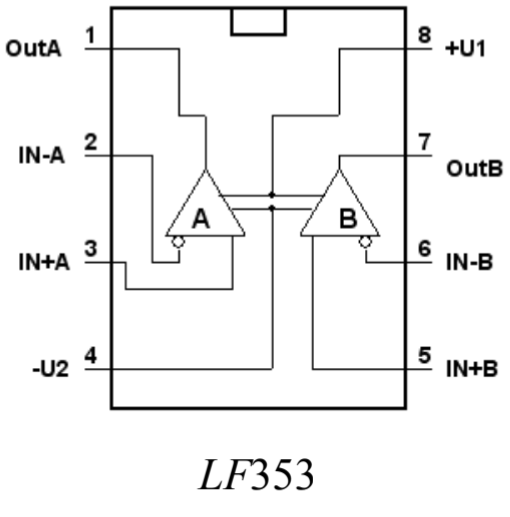
\includegraphics[width=4cm]{lf353.png}
        \label{real} %% метка рисунка для ссылки на него
        \end{center}
    \end{figure}

    \begin{figure}[H]
        \begin{center}
        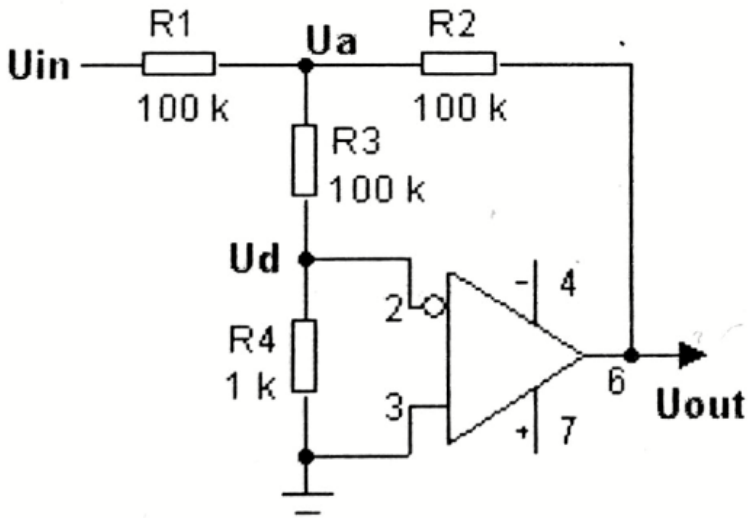
\includegraphics[width=6cm]{задание_1.png}
        \caption{Схема измерения коэффициента усиления.}
        \label{2} %% метка рисунка для ссылки на него
        \end{center}
    \end{figure}
    
    
\begin{enumerate}
    \item Соберем схему указанную на Рис. 1. Сопротивления резисторов $R_1 = R_2 = R_3 = 100 \; кОм ; \; R_4 = 1кОм$. Так что $\frac{R_3}{R_4} = 100$. 
    \item На вход подаем колебание с амплитудой $U_{in} = 2.5$ В и частотой $f = 15$ Гц. Измерим величину напряжения $U_a = 39.84 \;мВ$ и $ U_{out} = 3.92 \; В$.
    \item Рассчитаем коэффициент усиления по формуле:
    \begin{equation}
       A_0 = (1+\frac{R_3}{R_4})\cdot \frac{U_{out}}{U_a} \approx 9 \cdot 10^3
    \end{equation}

\end{enumerate}

\section{Задание №2. Амплитудно-частоотная характеристика ОУ.}

% \begin{figure}[H]
%     \begin{center}
%     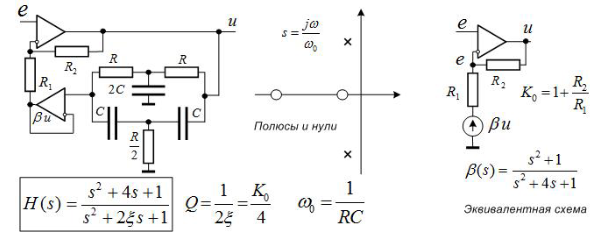
\includegraphics[width=12cm]{полосовой_фильтр.png}
%     \caption{Полосовой фильтр с двойным Т-мостом.}
%     \label{line} %% метка рисунка для ссылки на него
%     \end{center}
% \end{figure}

\begin{enumerate}
    \item Для схемы на рис. 1 снимем зависимость коэффициента усиления от частоты (АЧХ), используя формулу:
    
    \begin{equation}
        A(f) = \frac{U_out}{U_d}=\frac{U_out}{U_a}\cdot\frac{U_a}{U_d} = (1+\frac{R_3}{R_4})\cdot \frac{U_{out}}{U_a}
     \end{equation}

    \item Занесем полученные данные в таблицу 1.
    
     \begin{table}[H]
        \centering
        \begin{center}
        \end{center}
        \vspace{0.1cm}
        \label{tab:my_label}
        \begin{tabular}{|p{2cm}|p{1cm}|p{1cm}|p{1cm}|p{1cm}|p{1cm}|p{1cm}|p{1cm}|p{1cm}|p{1cm}|p{1cm}|}
            \hline
            f, Гц & 50    & 100   & 200 & 500 & 1k    & 2k    & 5k    & 10k    & 20k    & 50k    \\ 
            \hline
            $U_out$, В  & 5.00  & 5.00  & 5.00 & 4.99  & 4.98  & 4.92  & 4.54  & 3.66   & 2.38   & 1.00   \\
            \hline
            $U_a$, мВ                    & 36.5  & 41.5  & 57.5  & 101.2 & 181.0 & 329.0 & 723.0 & 1150.0 & 1480.0 & 1540.0 \\
            \hline
            A                        & 13836 & 12169 & 8783                     & 4980                     & 2779  & 1510  & 634   & 321    & 162    & 66     \\
            \hline
            lgf                         & 1.7   & 2     & 2.3                      & 2.7                      & 3     & 3.3   & 3.7   & 4      & 4.3    & 4.7    \\
            \hline
            20lfA, дБ                   & 83    & 82    & 79                       & 74                       & 69    & 64    & 56    & 50     & 44     & 36   \\
            \hline 
            \end{tabular}
            \caption{Зависимость коэффициента усиления от частоты.}
    \end{table}
    \item  Построим снятую зависимость в двойном логарифмическом масштабе, откладывая частоту в герцах, а коэффициент усиления в децибелах.
    
    \begin{figure}[H]
        \begin{center}
        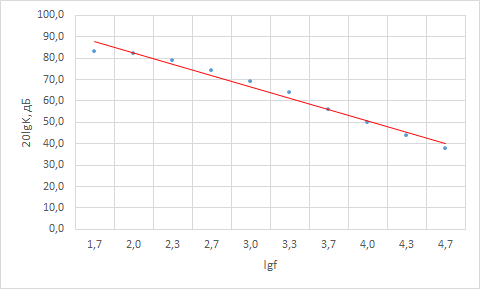
\includegraphics[width=10cm]{диаграма_1.png}
        \caption{АЧХ ОУ.}
        \label{2} %% метка рисунка для ссылки на него
        \end{center}
    \end{figure}
    

    \item Из рис. 2 получаем:
    
    \begin{equation}
        f_T \; \approx \; 10^{17} Гц, \; f_p \; \approx \; 10^{18} Гц.
     \end{equation}

    \end{enumerate}
\section{Задание №3. Неинвертирующий усилитель.}

\begin{figure}[H]
    \begin{center}
        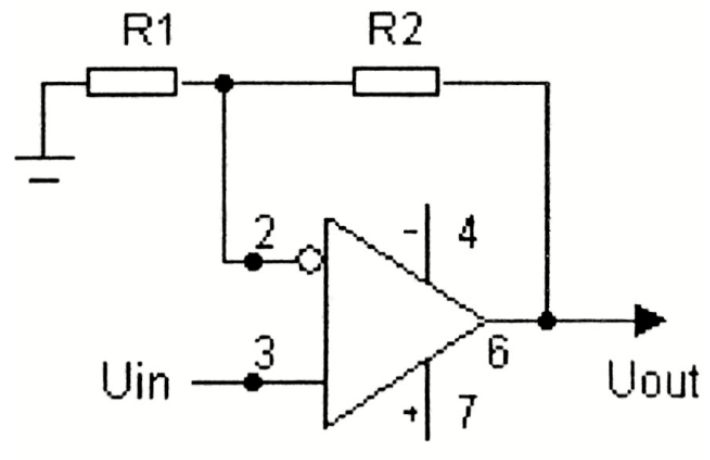
\includegraphics[scale = 0.5]{задание_3.png}
        \caption{Схема неинвертирующего усилителя.}
        \label{Sallen-Ki}
    \end{center}
\end{figure}

\begin{enumerate}
\item Соберем схему на рис. 3, выбрав $\frac{R_2}{R_1} = 100$
 
\item Определим входное напряжение сдвига ОУ: $U_{OS} =\frac{U_{out(dc)}}{1+\frac{R_2}{R_1}} \approx 2.7 мВ$.
\item Cнимем зависимость от частоты коэффициента усиления $K = \frac{U_{out}}{U_{in}}$ при $U_{вх} = 10мВ$.

\begin{table}[H]
    \centering
    \begin{center}
    \end{center}
    \vspace{0.1cm}
    \label{tab:my_label}
    \begin{tabular}{|p{2cm}|p{1cm}|p{1cm}|p{1cm}|p{1cm}|p{1cm}|p{1cm}|p{1cm}|p{1cm}|p{1cm}|p{1cm}|p{1cm}|p{1cm}|p{1cm}|p{1cm}|p{1cm}|}
        \hline
        f, Гц & 50    & 100   & 200 & 500 & 1k    & 2k    & 5k    & 10k    & 20k    & 50k  & 100k & 150k &300k &500k & 1M \\ 
        \hline
        $U_out$, В  & 2.46 & 2.45 & 2.45 & 2.45  & 2.45  & 2.44  & 2.39  & 2.32   & 2.06  & 1.32 & 0.77  & 0.55 & 0.29 & 0.19 & 0.09\\
        \hline
        K    & 246 & 245 & 245  & 245  & 245   & 244   & 239    & 232    & 206   & 132 & 77 & 55 &  29 & 19 & 9 \\
        \hline
        lnf     & 3.9   & 4.6  & 5.3  & 6.2 & 6.9  & 7.6 & 8.5   & 9.2  & 9.9 &  10.8 & 11.5 & 11.9 & 12.6 & 13.1 & 13.8 \\
        \hline
        20lnK, дБ   & 110   & 110  & 110 & 110 &  110  & 110  & 109.5 &  109 & 107  & 98 & 87 & 80 & 67 & 59 & 44 \\
        \hline 
        \end{tabular}
        \caption{Зависимость коэффициента усиления K(f).}
\end{table}


\begin{figure}[H]
    \begin{center}
        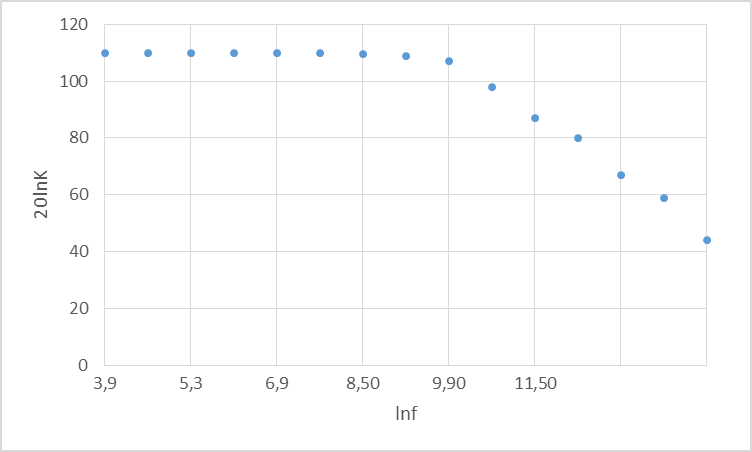
\includegraphics[scale = 0.6]{диаграма_2.png}
        \caption{Зависимость коэффициента усиления K(f)}
        \label{Sallen-Ki}
    \end{center}
\end{figure}

\item  Из рис. 4 определим граничную частоту $F_p$ по уровню 0.7 относительно коэффициента усиления на низких частотах. Получим $F_p \approx 35 кГц$.
\item Проверим, что коэффициент усиления на низких частотаз ($f < F_p$) и граничная частота усилителя удовлетворяют соотношениям:

\begin{equation}
   K_0 = \frac{1}{\beta} = 1 + \frac{R_2}{R_1} = 101 \\
   F_p = \beta \cdot f_T = 10^{15} \\
   \beta = \frac{R_1}{R_1 + R_2} = 0.01 
 \end{equation}

 \item Включи ОУ по схеме повторителя ($R_1 = \infty, R_2 = 0$). Измерим коэффициент передачи и граничную частоту усилителя. Определим на частоте $f = 1.5 кГц$ максимальную амплитуду неискаженного сигнала и характер искажений, возникающих при дальнейшем увеличении амплитуды входного сигнала. Получим $U_{m-out} \approx 8$ В. 


\begin{table}[H]
    \centering
    \begin{center}
    \end{center}
    \vspace{0.1cm}
    \label{tab:my_label}
    \begin{tabular}{|p{2cm}|p{1cm}|p{1cm}|p{1cm}|p{1cm}|p{1cm}|p{1cm}|p{1cm}|p{1cm}|p{1cm}|p{1cm}|p{1cm}|p{1cm}|p{1cm}|p{1cm}|p{1cm}|p{1cm}|p{1cm}|}
        \hline
        f, Гц & 50 & 100 & 200 & 500 & 1k & 2k & 5k & 10k & 20k & 1M  & 2M & 2.5M & 3M & 5M & 10M & 15M & 20M \\ 
        \hline
        K    & 1.0 & 1.01 & 1.02  & 1.01 & 1.02 & 1.02  & 1.01 & 1.01 & 1.00 & 1.01 & 1.02 & 1.02 &  1.02 & 1.01 & 1.02 & 0.99 & 0.88 \\
        \hline
        lnf     & 3.9   & 4.6  & 5.3  & 6.2 & 6.9  & 7.6 & 8.5   & 9.2  & 9.9 &  13.8 & 14.5 & 14.7 & 14.9 & 15.4 & 16.1 & 16.5 & 16.8 \\
        \hline
        20lnK, дБ   &  0  & 0.2  & 0.4 & 0.2 &  0.4  & 0.4  & 0.2 &  0.2 & 0 & 0.2 & 0.4 & 0.4 & 0.4 & 0.2 & 0.4 &-0.2& -2.6\\
        \hline 
        \end{tabular}
        \caption{Зависимость коэффициента усиления K(f) повторителя.}
\end{table}

\begin{figure}[H]
    \begin{center}
        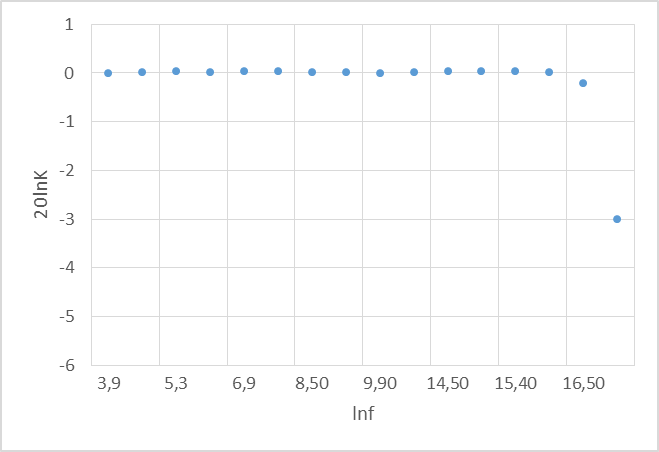
\includegraphics[scale = 0.6]{lbfuhfvf_3.png}
        \caption{Зависимость коэффициента усиления K(f) повторителя}
        \label{Sallen-Ki}
    \end{center}
\end{figure}

\item Из рис. 5 получаем, что граничная частота равна $f \approx 13$МГц. Сравним с расчетом по формуле $U_{m-out} = \frac{V_{max}}{2 \pi f} \approx 4$В.

\end{enumerate}
\section{Задание №5. Разностный усилитель. }


\begin{figure}[H]
    \begin{center}
        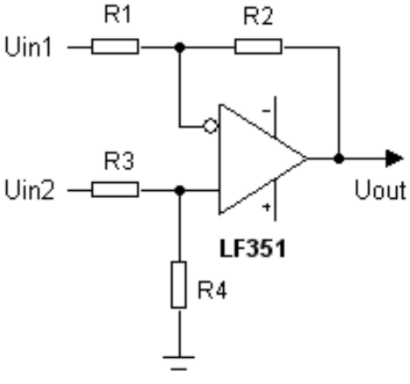
\includegraphics[scale = 0.6]{задание_5.png}
        \caption{Схема разностного усилителя}
        \label{Sallen-Ki}
    \end{center}
\end{figure}

\begin{enumerate}
    \item Соберем схему, изображенную на рис. 5. Здесь $\frac{R_2}{R_1} = 10, R_3 = R_1, R_4 =R_2$.
    \item Измерим коэффициент усиления по $U_{in1} $ и $U_{in2}$. 
     
    \begin{table}[H]
        \centering
        \begin{center}
        \end{center}
        \vspace{0.1cm}
        \label{tab:my_label}
        \begin{tabular}{|p{2cm}|p{1cm}|p{1cm}|p{1cm}|p{1cm}|p{1cm}|p{1cm}|p{1cm}|p{1cm}|p{1cm}|}
            \hline
            f, Гц & 50 & 100  & 500 & 1k & 3k & 10k & 100k & 500k  & 1M  \\ 
            \hline
            $K_1$   & 35 &  10  &  10 & 10  & 10  & 10 &  9 &  5 & 2 \\
            \hline
            $K_2$  & 10 &   10 &   10  & 10  & 10  & 9 &  5 &  8 & 2 \\
            \hline
            \end{tabular}
            \caption{Зависимость коэффициента усиления K.}
    \end{table}

    \item  Объединив входы, убедились, что коэффициент усиления общего сигнала близок к нулю.
    \item $U_{out} = \frac{R_2}{R_1}\cdot(U_{in2} - U_{in1}) \approx 1$ В.

\end{enumerate}

\subsection{Вывод:}
Изучили устройство операционного усилителя. Разобрали различные схемы усилителей.
\end{document}